\documentclass[12pt]{beamer}
\newenvironment{ConCodigo}[1]
  {\begin{frame}[fragile,environment=ConCodigo]{#1}}
  {\end{frame}}
\graphicspath{{Imagenes/}{../Imagenes/}}
\usepackage[utf8]{inputenc}
\usepackage[spanish]{babel}
\usepackage{hyperref}
\usepackage{etex}
\reserveinserts{28}
\usepackage{amsmath}
\usepackage{amsthm}
\usepackage{mathtools}
\usepackage{multicol}
\usepackage{multirow}
\usepackage{tabulary}
%\usepackage{tabularx}
\usepackage{booktabs}
\usepackage{nccmath}
\usepackage{biblatex}
\usepackage{epstopdf}
\usepackage{graphicx}
\usepackage{siunitx}
\sisetup{scientific-notation=true}
%\usepackage{fontspec}
\usepackage{lmodern}
\usepackage{float}
\usepackage[format=hang, font=footnotesize, labelformat=parens]{caption}
\usepackage[autostyle,spanish=mexican]{csquotes}
\usepackage{standalone}
\usepackage{tikz}
\usepackage[siunitx]{circuitikz}
\usetikzlibrary{arrows,patterns,shapes}
\usetikzlibrary{decorations.markings}
\usetikzlibrary{arrows}
\usepackage{color}
%\usepackage{beton}
%\usepackage{euler}
%\usepackage[T1]{fontenc}
\usepackage[sfdefault]{roboto}  %% Option 'sfdefault' only if the base font of the document is to be sans serif
\usepackage[T1]{fontenc}
\renewcommand*\familydefault{\sfdefault}
\DeclareGraphicsExtensions{.pdf,.png,.jpg}
\usepackage{hyperref}
\renewcommand {\arraystretch}{1.5}
\newcommand{\python}{\texttt{python}}
\usefonttheme[onlymath]{serif}
\setbeamertemplate{navigation symbols}{}
\usetikzlibrary{patterns}
\usetikzlibrary{decorations.markings}
\tikzstyle{every picture}+=[remember picture,baseline]
%\tikzstyle{every node}+=[inner sep=0pt,anchor=base,
%minimum width=2.2cm,align=center,text depth=.15ex,outer sep=1.5pt]
%\tikzstyle{every path}+=[thick, rounded corners]
\setbeamertemplate{caption}[numbered]
\newcommand{\ptm}{\fontfamily{ptm}\selectfont}
%Se usa la plantilla Warsaw modificada con spruce
\mode<presentation>
{
  \usetheme{Warsaw}
  \setbeamertemplate{headline}{}
  \useoutertheme{default}
  \usecolortheme{beaver}
  \setbeamercovered{invisible}
}
\AtBeginSection[]
{
\begin{frame}<beamer>{Contenido}
\normalfont\mdseries
\tableofcontents[currentsection]
\end{frame}
}

\usepackage{listings}
\lstset{ %
language=Python,                % choose the language of the code
basicstyle=\small,       % the size of the fonts that are used for the code
numbers=left,                   % where to put the line-numbers
numberstyle=\small,      % the size of the fonts that are used for the line-numbers
stepnumber=1,                   % the step between two line-numbers. If it is 1 each line will be numbered
numbersep=5pt,                  % how far the line-numbers are from the code
backgroundcolor=\color{white},  % choose the background color. You must add \usepackage{color}
showspaces=false,               % show spaces adding particular underscores
showstringspaces=false,         % underline spaces within strings
showtabs=false,                 % show tabs within strings adding particular underscores
frame=single,   		% adds a frame around the code
tabsize=2,  		% sets default tabsize to 2 spaces
captionpos=b,   		% sets the caption-position to bottom
breaklines=true,    	% sets automatic line breaking
breakatwhitespace=false,    % sets if automatic breaks should only happen at whitespace
escapeinside={\%},          % if you want to add a comment within your code
stringstyle =\color{magenta},
keywordstyle = \color{blue},
commentstyle = \color{green},
identifierstyle = \color{red}
}
\begin{document}
\title{Tema 2 - Operaciones matem\'{a}ticas b\'{a}sicas}
\subtitle{C\'{a}lculo de ra\'{i}ces II}
%\subsubtitle{Curso de F\'{i}sica Computacional}
\author{M. en C. Gustavo Contreras May\'{e}n}
%\email{curso.fisica.comp@gmail.com}
%\ptsize{10}
\maketitle
\fontsize{14}{14}\selectfont
\spanishdecimal{.}
\begin{frame}{Contenido}
;\tableofcontents[pausesections]
\end{frame}
\section{M\'{e}todo de Newton-Raphson}
\begin{frame}
\frametitle{M\'{e}todo de Newton-Raphson}
Este m\'{e}todo se basa en el desarrollo de la serie de Taylor de $f(x)$ alrededor de $x$
\[ f(x) = f(x_{0}) + f'(x_{0}) (x-x_{0}) + O(x-x_{0})^{2} \]
Como se puede evidenciar, el pequeño detalle del m\'{e}todo es que se tiene que usar $f'(x)$, por tanto, los problemas a resolver con este algoritmo, deber\'{a} de contemplarse que la derivada sea f\'{a}cil de calcularse.
\end{frame}
\begin{frame}
Para resolver la ecuaci\'{o}n $f(x)=0$, se sustituye en la serie de Taylor
\[ 0 = f(x_{0}) + f'(x_{0}) (x-x_{0}) + O(x-x_{0})^{2} \]
Si $x_{0}$ est\'{a} cerca de la ra\'{i}z de x, entonces sucede lo siguiente:
\begin{enumerate}[<+->]
\item $(x-x_{0})$ es pequeño.
\item $(x-x_{0})^{2}$ es m\'{a}s pequeño.
\item $(x-x_{0})^{3}$ es todav\'{i}a mucho m\'{a}s pequeño.
\end{enumerate}
\end{frame}
\begin{frame}
Al ignorar los t\'{e}rminos de orden superior, tenemos que
\[ f(x_{0}) + f'(x_{0})(x-x_{0}) \simeq 0\]
ordenando los t\'{e}rminos
\[ x \simeq x_{0} - \dfrac{f(x_{0})}{f'(x_{0})} \]
\end{frame}
\subsection{Algoritmo}
\begin{frame}
\frametitle{Algortimo}
Al iterar la expresi\'{o}n anterior:
\[ \boxed{ x_{n+1} = x_{n} - \dfrac{f(x_{n})}{f'(x_{n})} }\]
Esto significa que si tenemos un punto de inicio para $x_{0}$, entonces podemos iterar la expresi\'{o}n hasta encontrar la ra\'{i}z $x$ estableciendo una tolerancia.
\end{frame}
\begin{frame}
\frametitle{Ejemplo}
Tenemos la funci\'{o}n $f(x)=x^{2}$, sabemos que hay una ra\'{i}z en el origen, por lo que
\[ \dfrac{f(x)}{f'(x)} = \dfrac{x}{2}\]
Al aplicar la f\'{o}rmula de Newton-Raphson con el punto de inicio en $x=0.1$, obtenemos:
\end{frame}
\begin{frame}
\[ \begin{split} 
x \leftarrow& x - \dfrac{f(x)}{f'(x)} = 0.1 - \dfrac{0.1}{2} = 0.1 - 0.05 = 0.05 \\
\visible<2->{x \leftarrow& x - \dfrac{f(x)}{f'(x)} = 0.25} \\
\visible<3->{x \leftarrow& x - \dfrac{f(x)}{f'(x)} = 0.125} \\
\visible<4->{x \leftarrow& x - \dfrac{f(x)}{f'(x)} = 0.00625} \\
\end{split} \]
\visible<5->{Lo que nos indica que nos estamos acercando a la ra\'{i}z en $x=0$}
\end{frame}
\begin{frame}
\frametitle{Representaci\'{o}n gr\'{a}fica}
Podemos interpretar que $x_{n+1}$ es el punto en donde la tangente de $f(x_{n})$ cruza el eje de las $x$:
\begin{center}
\begin{tikzpicture}[font=\small, scale=0.8]
\draw [->] (0,0) -- (7,0);
\draw [<->] (0,-3) -- (0,3);
\draw [red] (1,3) .. controls (1.5,0.5) and (5,-2) .. (6.5,-2);
\draw (1,-0.3) node {$x_{0}$};
\draw (1,3.3) node {$f(x_{0})$};
\draw [dashed] (1.2,0) -- (1.2,2.35);
\draw (0.8,3.1) -- (2.35,-0.1);
\draw [dashed] (2.3,0) -- (2.3,0.58);
%\draw [dashed] (6.3,0) -- (6.3,-1.98);
%\draw (1.2,2.35) -- (6.3,-1.98);
%\draw  (3,3) node {1a. interpolaci\'{o}n};
%\draw [->] (3,2.6) -- (2,2);
%\draw  (5,1) node {1a. aproximaci\'{o}n};
%\draw [->] (5,0.6) -- (4.1,0.1);
%\draw [dashed] (4,0) -- (4,-0.9);
%\draw [dashed] (1,0) -- (1,2.7); 
\end{tikzpicture}
\end{center}
\end{frame}
\begin{frame}
\frametitle{¿Qu\'{e} tan bien funciona el m\'{e}todo}
Consideremos la funci\'{o}n
\[ g(x) = x^{1/3} \]
y sea el punto de inicio $x=0.1$
\begin{figure}
	\centering
	\visible<2-> {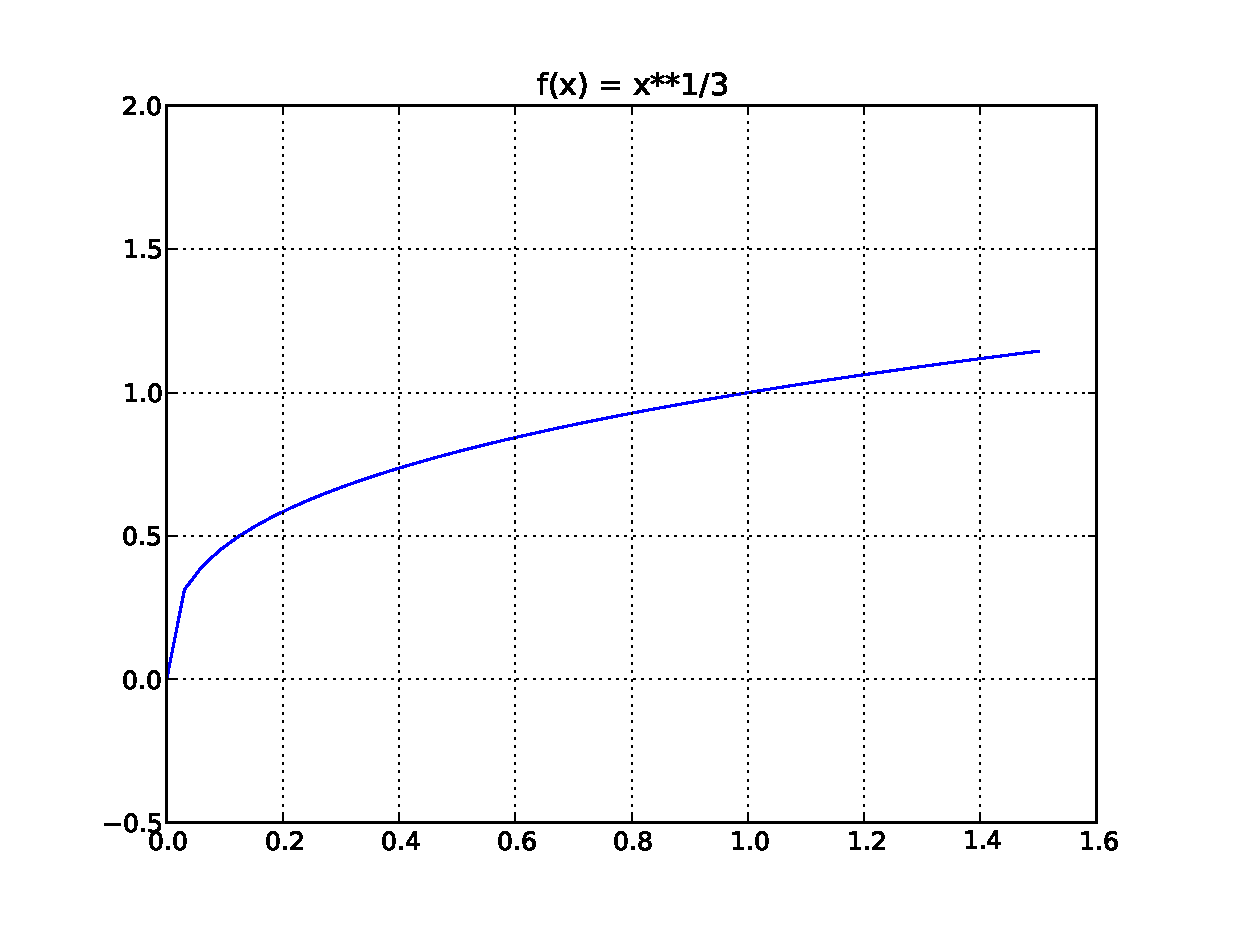
\includegraphics[scale=0.4]{raices07.eps}}
\end{figure}
\end{frame}
\begin{frame}
\frametitle{Ejercicio}
Encontrar la ra\'{i}z positiva m\'{a}s pequeña de
\[ f(x) = x^{4} - 6.4 x^{3} + 6.45x^{2} + 20.538x - 31.752\]
\begin{figure}
	\centering
	\visible<2-> {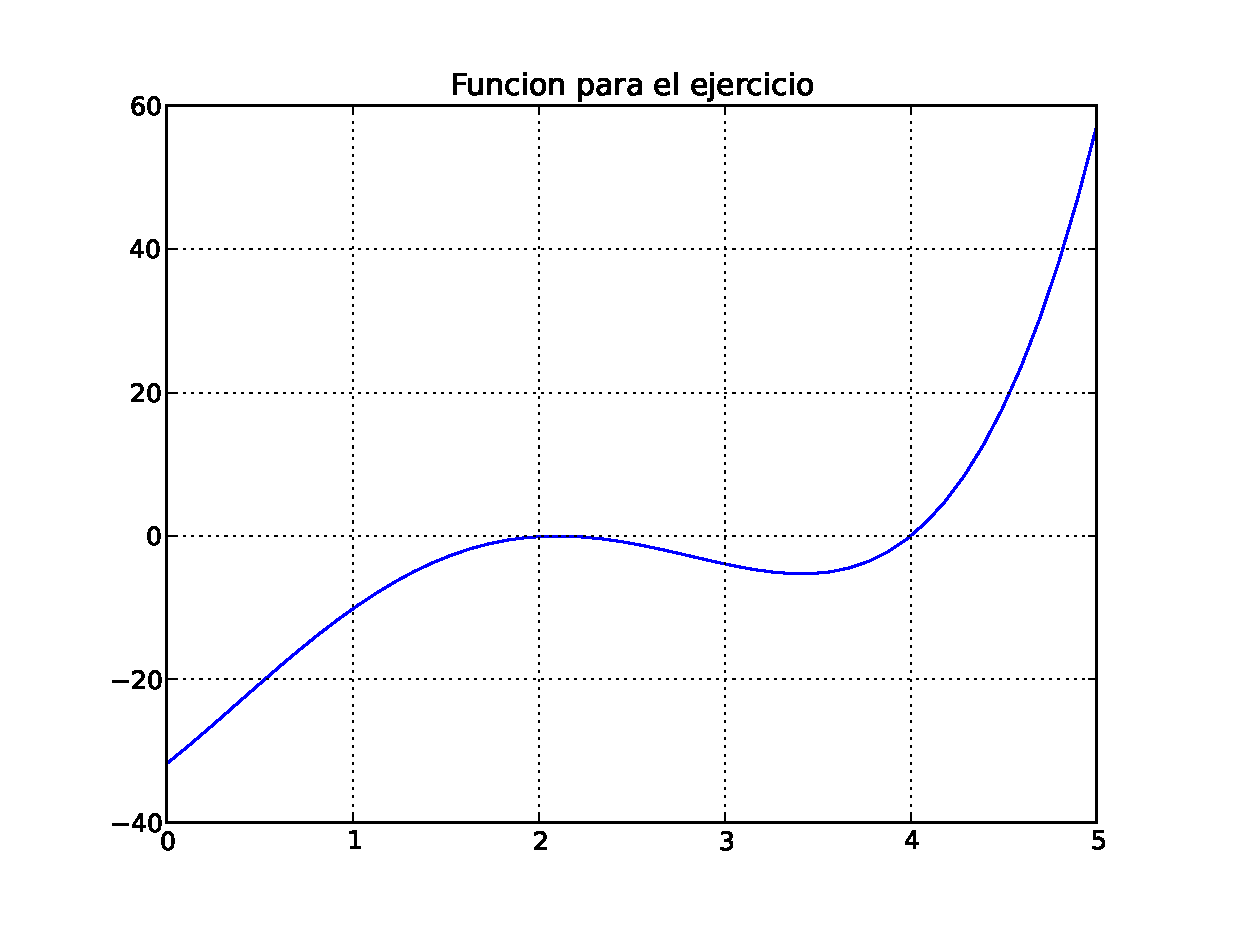
\includegraphics[scale=0.4]{raices08.eps}}
\end{figure}
\end{frame}
\begin{frame}[fragile]
\begin{lstlisting}
def f(x): return x**4 - 6.4*x**3 + 6.45*x**2 + 20.538*x - 31.752
def df(x): return 4.0*x**3 - 19.2*x**2 + 12.9*x + 20.538

def newtonRaphson(x,tol=1e-05):
    for i in range(50):
        dx = -f(x)/df(x)
        x = x + dx
        if abs(dx) < tol: return x,i
    print 'Son demasiadas iteraciones\n'

raiz,numIter = newtonRaphson(2.0)

print 'Raiz =',raiz
print 'Numero de iteraciones =',numIter
\end{lstlisting}
\end{frame}
\begin{frame}
\frametitle{Ejercicio para casa}
Calcular la ra\'{i}z positiva m\'{a}s pequeña de
\[y = \tan(x) - 0.5 x\]
mediante el m\'{e}todo de Newton-Raphson, con una tolerancia de $\epsilon=0.001$
\end{frame}
\begin{frame}
Obtener la primera derivada de una funci\'{o}n dada puede ser una tarea complicada.
\\
\bigskip
En tal caso, se puede evaluar $f'(x_{i})$ mediante una aproximaci\'{o}n por diferencias en vez de la forma anal\'{i}tica.
\\
\bigskip
Se puede aproximar $f'(x_{i-1})$ mediante la aproximaci\'{o}n por diferencias hacia adelante:
\[ f'(x_{i-1}) = \dfrac{f(x_{i-1}+h) - f(x_{i-1})}{h}\]
donde $h$ es un valor pequeño.
\end{frame}
\section{M\'{e}todo de la falsa posici\'{o}n}
\begin{frame}
\frametitle{M\'{e}todo de la falsa posici\'{o}n}
Este m\'{e}todo es parecido al de bisecci\'{o}n, ya que el intervalo que contiene a la ra\'{i}z se va reduciendo.
\\
\bigskip
En vez de bisectar de manera mon\'{o}tona el intervalo, se utiliza una interpolaci\'{o}n lineal ajustada a dos puntos extremos para encontrar la
aproximaci\'{o}n de la ra\'{i}z.
\end{frame}
\begin{frame}
La funci\'{o}n est\'{a} bien aproximada por la interpolaci\'{o}n lineal, con lo que las ra\'{i}ces tendr\'{a}n una buena precisi\'{o}n; la iteraci\'{o}n converger\'{a} m\'{a}s r\'{a}pido que como ocurre con el m\'{e}todo de
bisecci\'{o}n.
\end{frame}
\begin{frame}
Dado un intervalo $[a,c]$ que contenga a la raíz, la funci\'{o}n lineal que pasa por $(a,f(a))$ y $(c,f(c))$ se escribe como:
\[ y = f(a) + \dfrac{f(c)-f(a)}{c-a}(x-a) \]
de donde se despeja $x$:
\[ x = a + \dfrac{c-a}{f(c)-f(a)}(y-f(a)) \]
\end{frame}
\begin{frame}
La coordenada $x$ en donde la l\'{i}nea intersecta al eje $x$ se determina al hacer $y=0$ en la ecuaci\'{o}n anterior, por tanto:
\[ b = a - \dfrac{c-a}{f(c)-f(a)}f(a) = \dfrac{af(c)-cf(a)}{f(c)-f(a)} \]
\end{frame}
\begin{frame}
Despu\'{e}s de encontrar $b$, el intervalo $[a,c]$ se divide en $[a,b]$ y $[b,c]$.
\\
\bigskip
Si $f(a)f(b) \leq 0$, la ra\'{i}z se encuentra en $[a,b]$; en caso contrario, est\'{a} en $[b,c]$. Los extremos del nuevo intervalo que contiene a la ra\'{i}z se renombran para el siguiente paso como $a$ y $c$.
\\
\bigskip
El procedimiento de interpolaci\'{o}n se repite hasta que las ra\'{i}ces estimadas convergen.
\end{frame}
\begin{frame}[fragile]
\frametitle{M\'{e}todo de la falsa posici\'{o}n}
\begin{center}
\begin{tikzpicture}[font=\small]
\draw [->] (0,0) -- (7,0);
\draw [<->](0,-3) -- (0,3);
\draw [red] (1,3) .. controls (1.5,0.5) and (5,-2) .. (6.5,-2);
\draw (1,-0.3) node {x=a};
\draw (6,0.3) node {x=c};
\draw [dashed] (1.2,0) -- (1.2,2.35);
\draw [dashed] (6.3,0) -- (6.3,-1.98);
\draw (1.2,2.35) -- (6.3,-1.98);
\draw  (3,3) node {1a. interpolaci\'{o}n};
\draw [->] (3,2.6) -- (2,2);
\draw  (5,1) node {1a. aproximaci\'{o}n};
\draw [->] (5,0.6) -- (4.1,0.1);
\draw [dashed] (4,0) -- (4,-0.9);
%\draw [dashed] (1,0) -- (1,2.7); 
\end{tikzpicture}
\end{center}
\end{frame}
\begin{frame}[fragile]
\frametitle{M\'{e}todo de la falsa posici\'{o}n}
\begin{center}
\begin{tikzpicture}[font=\small]
\draw [->] (0,0) -- (7,0);
\draw [<->] (0,-3) -- (0,3);
\draw [red] (1,3) .. controls (1.5,0.5) and (5,-2) .. (6.5,-2);
\draw (1,-0.3) node {x=a};
\draw (6,0.3) node {x=c};
\draw [dashed] (1.2,0) -- (1.2,2.35);
\draw [dashed] (6.3,0) -- (6.3,-1.98);
\draw (1.2,2.35) -- (6.3,-1.98);
\draw (1.2,2.35) -- (4,-0.9);
\draw  (4,2) node {2a. interpolaci\'{o}n};
\draw [->] (4,1.6) -- (2.5,1);
\draw  (6,1) node {2a. aproximaci\'{o}n};
\draw [->] (5.5,0.8) -- (3.3,0.1);
\draw [dashed] (4,0) -- (4,-0.9);
\draw [dashed] (3.25,0) -- (3.25,-0.43); 
\end{tikzpicture}
\end{center}
\end{frame}
\begin{frame}
La desventaja de este m\'{e}todo es que aparecen extremos fijos: uno de los extremos de la sucesi\'{o}n de intervalos no se mueve del punto original, por lo que las aproximaciones a la raíz, denotadas por $b_{1}$, $b_{2}$, $b_{3}$, etc. convergen a la ra\'{i}z exacta solamente por un lado.
\\
\bigskip
Los extremos fijos no son deseables debido a que hacen m\'{a}s lenta la convergencia, en particular cuando el intervalo es grande o cuando la funci\'{o}n
se desv\'{i}a de manera significativa de una l\'{i}nea recta en el intervalo.
\\
\bigskip
¿Qu\'{e} podemos hacer al respecto?
\end{frame}
\section{M\'{e}todo de la falsa posici\'{o}n modificado}
\begin{frame}
\frametitle{M\'{e}todo de la falsa posici\'{o}n modificado}
En este m\'{e}todo, el valor de $f$ en un punto fijo se divide a la mitad si este punto se ha repetido m\'{a}s de dos veces.
\\
\bigskip
El extremo que se repite se llama extremo fijo. La excepci\'{o}n para esta regla es que para $i=2$, el valor de $f$ en un extremo se divide entre 2 de
inmediato si no se mueve.
\end{frame}
\begin{frame}[fragile]
\frametitle{M\'{e}todo de falsa posici\'{o}n modificado}
\begin{center}
\begin{tikzpicture}[font=\small]
\draw [->] (0,0) -- (7,0);
\draw [<->] (0,-3) -- (0,3);
\draw [red] (1,3) .. controls (1.5,0.5) and (5,-2) .. (6.5,-2);
\draw (1,-0.3) node {x=a};
\draw (6,0.3) node {x=c};
\draw [dashed] (1.2,0) -- (1.2,2.35);
\draw [dashed] (6.3,0) -- (6.3,-1.98);
\draw (1.2,2.35) -- (6.3,-1.98);
\draw  (3,3) node {1a. interpolaci\'{o}n};
\draw [->] (3,2.6) -- (2,2);
\draw  (5,1) node {1a. aproximaci\'{o}n};
\draw [->] (5,0.6) -- (4.1,0.1);
\draw [dashed] (4,0) -- (4,-0.9);
%\draw [dashed] (1,0) -- (1,2.7); 
\end{tikzpicture}
\end{center}
\end{frame}
\begin{frame}[fragile]
\frametitle{M\'{e}todo de la falsa posici\'{o}n modificado}
\begin{center}
\begin{tikzpicture}[font=\small]
\draw [->] (0,0) -- (7,0);
\draw [<->] (0,-3) -- (0,3);
\draw [red] (1,3) .. controls (1.5,0.5) and (5,-2) .. (6.5,-2);
\draw (1,-0.3) node {x=a};
\draw (6,0.3) node {x=c};
\draw [dashed] (1.2,0) -- (1.2,2.35);
\draw [dashed] (6.3,0) -- (6.3,-1.98);
\draw (1.2,2.35) -- (6.3,-1.98);
\draw (1.2,1.3) -- (4,-0.9);
\draw  (4,2) node {2a. interpolaci\'{o}n};
\draw [->] (4,1.6) -- (1.8,1);
\draw  (6,1) node {2a. aproximaci\'{o}n};
\draw [->] (5.5,0.8) -- (3.1,0.1);
\draw [dashed] (4,0) -- (4,-0.9);
%\draw [dashed] (3.25,0) -- (3.25,-0.43); 
\end{tikzpicture}
\end{center}
\end{frame}
\section{M\'{e}todo de la secante}
\begin{frame}
\frametitle{M\'{e}todo de la secante}
A diferencia del m\'{e}todo de Newton, el valor de $f'$ se aproxima utilizando dos valores de iteraciones consecutivas de $f$. Con lo que se elimina la necesidad de evaluar tanto a $f$ como a $f'$ en cada iteraci\'{o}n.
\end{frame}
\begin{frame}
Las aproximaciones sucesivas para la ra\'{i}z en el m\'{e}todo de la secante est\'{a}n dadas por:
\[ x_{n} = x_{n-1} - y_{n-1} \dfrac{x_{n-1} - x_{n-2}}{y_{n-1}- y_{n-1}}, \hspace{1cm} n=2,3,\ldots \]
donde $x_{0}$ y $x_{1}$ son dos suposiciones iniciales para comenzar la iteraci\'{o}n.
\end{frame}
\begin{frame}[fragile]
\frametitle{M\'{e}todo de la secante}
\begin{center}
\begin{tikzpicture}[font=\small]
\draw [->] (0,0) -- (7.5,0);
\draw [->] (0,0) -- (0,4);
\draw [red](7,3.5) .. controls (6.3,2) and (4.5,0.3) .. (1,0);
%\draw (6.3,2) circle (0.1);
%\draw (4.5,0.3) circle (0.1);
\draw [dashed] (6.8,3.1) -- (6.8,0);
\draw (6.6,-0.2) node {$x_{0}$};
\draw (6.6, 3.3) node {$f_{0}$};
\draw [dashed] (5.5,1.65) -- (5.5,0);
\draw (5.25,-0.2) node {$x_{1}$};
\draw (5.25, 1.8) node {$f_{1}$};
\draw (6.8,3.1) -- (4.1,0);
\draw (4,-0.2) node {$x_{2}$};
\draw [dashed] (4.1,0) -- (4.1,0.8);
\draw (3.9, 1) node {$f_{2}$};
\draw (5.5,1.65) -- (2.9,0);
\draw (2.8,-0.2) node {$x_{3}$};
\end{tikzpicture}
\end{center}
\end{frame}
\end{document}
